\documentclass[a4paper, twoside]{article}

%% Language and font encodings
\usepackage[english]{babel}
\usepackage[utf8x]{inputenc}
\usepackage[T1]{fontenc}

%% Sets page size and margins
\usepackage[a4paper,top=3cm,bottom=2cm,left=3cm,right=3cm,marginparwidth=1.75cm]{geometry}

%% Useful packages
\usepackage{amsmath}
\usepackage{graphicx}
\graphicspath{ {./images/} }
\usepackage[colorinlistoftodos]{todonotes}
\usepackage[colorlinks=true, allcolors=black]{hyperref}
\usepackage{caption}


\title{Logiciel Spécialisé R}
\author{Sébastien \textsc{Calvignac} \linebreak Kassim \textsc{Kone}}
% Update supervisor and other title stuff in title/title.tex

\usepackage{Sweave}
\begin{document}
\Sconcordance{concordance:rapport.tex:rapport.Rnw:%
1 23 1 1 0 195 1}

\begin{titlepage}

\newcommand{\HRule}{\rule{\linewidth}{0.5mm}} % Defines a new command for the horizontal lines, change thickness here

%----------------------------------------------------------------------------------------
%	LOGO SECTION
%----------------------------------------------------------------------------------------


\includegraphics[width=5cm]{UGAlogo.png}\\[1cm] % Include a department/university logo - this will require the graphicx package
 
%----------------------------------------------------------------------------------------

\center % Center everything on the page

%----------------------------------------------------------------------------------------
%	HEADING SECTIONS
%----------------------------------------------------------------------------------------

\textsc{\LARGE Compte rendu de projet}\\[1.5cm] % Name of your university/college
\textsc{\Large Université Grenoble Alpes}\\[0.5cm] % Major heading such as course name
\textsc{\large Informatique, Mathématiques et
Mathématiques Appliquées de Grenoble}\\[0.5cm] % Minor heading such as course title

%----------------------------------------------------------------------------------------
%	TITLE SECTION
%----------------------------------------------------------------------------------------
\makeatletter
\HRule \\[0.4cm]
{ \huge \bfseries \@title}\\[0.4cm] % Title of your document
\HRule \\[1.5cm]
 
%----------------------------------------------------------------------------------------
%	AUTHOR SECTION
%----------------------------------------------------------------------------------------
\vfill
\begin{minipage}{0.4\textwidth}
\begin{flushleft} \large
\emph{Auteur:}\\
\@author % Your name
\end{flushleft}
\end{minipage}
~
\begin{minipage}{0.4\textwidth}
\begin{flushright} \large
%\emph{Supervisor:} \\
%Prof. Lily Smith \\[1.2em] % Supervisor's Name
\emph{Enseignant :} \\
M. Rémy \textsc{Drouilhet} % second marker's name
\end{flushright}
\end{minipage}\\[2cm]
\makeatother

% If you don't want a supervisor, uncomment the two lines below and remove the section above
%\Large \emph{Author:}\\
%John \textsc{Smith}\\[3cm] % Your name

%----------------------------------------------------------------------------------------
%	DATE SECTION
%----------------------------------------------------------------------------------------

{\large \today}\\[2cm] % Date, change the \today to a set date if you want to be precise

\end{titlepage}

\tableofcontents
\clearpage
\section{Résumé}
Dans le cadre du Master de Statistique et Sciences des Données, nous nous 
formons à la génération de rapport et de dévéloppement en R avec M. Drouilhet. 
Nous allons nous intéresser dans ce rapport au sujet de l'analyse spatiale de 
données géolinguistiques et géographiques. Et dans un second temps à 
l'experience de développement d'un package R pour une application Shiny.

\section{Géomatique}
\subsection{Définition}
La géomatique regroupe l'ensemble des outils mathématiques permettant 
d'acquérir,  représenter et analyser des données géographiques.

\begin{figure}[h]
\caption{Visualisation de couches de données géographiques}
\centering
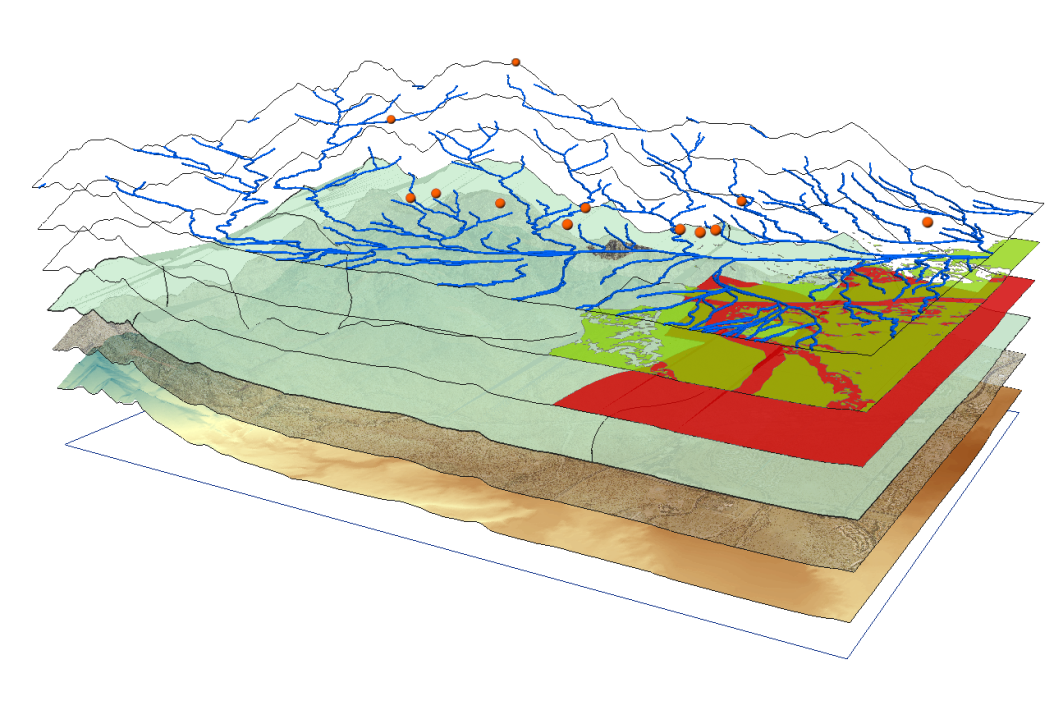
\includegraphics[width=0.6\textwidth]{couchesGeo}
\end{figure}

\subsection{Occitanie}
Occitanie est une zone géographique au sud de la France qui a sa propre langue 
appelé l'occitan avec différent dialectes. 

\begin{figure}[h]
\caption{La région d’Occitanie}
\centering
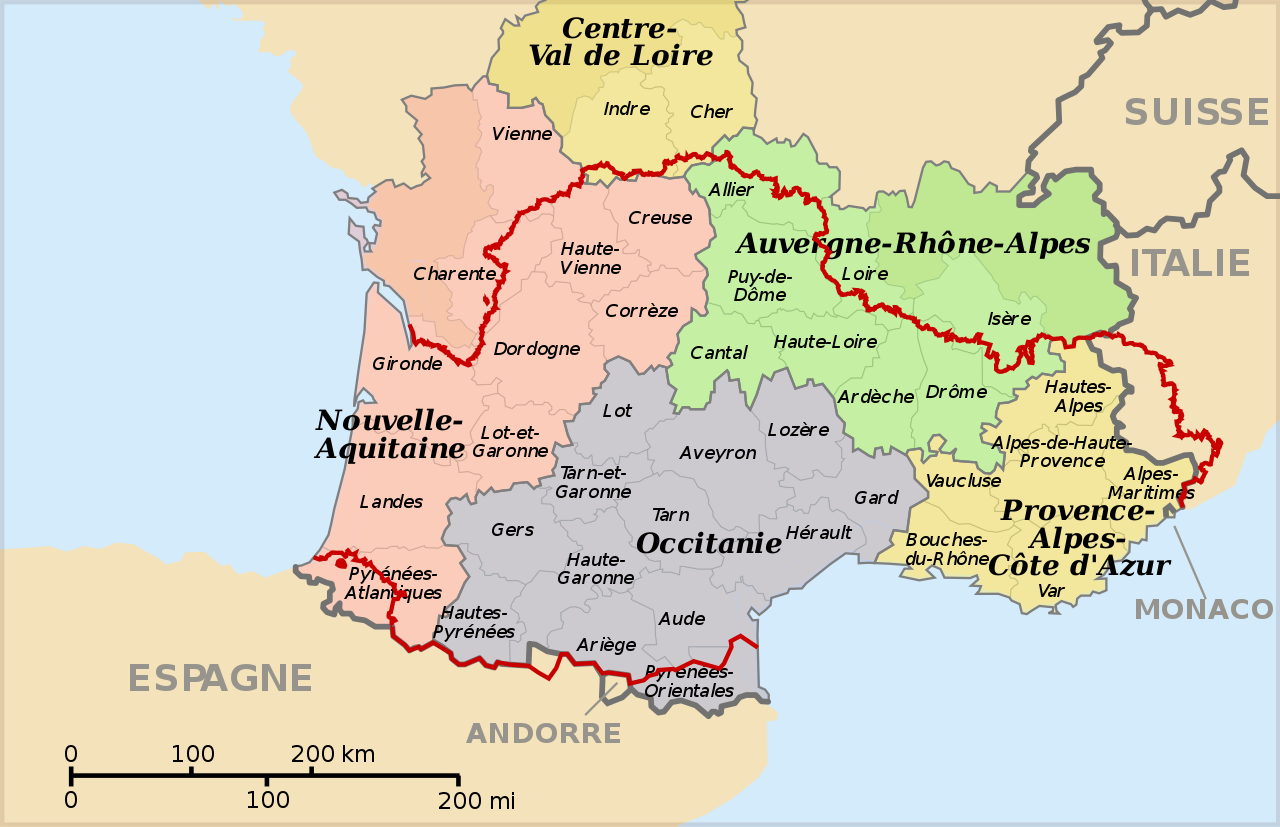
\includegraphics[width=0.6\textwidth]{occitan}
\end{figure}

\subsection{Données}
Un sondage qui date du début du 20ème siècle, a enregistré quel mots était 
utilisé dans chaque village pour exprimer une même idée. Avec ces données nous 
pouvons visualiser quels mots étaient utilisé dans l'espace géographique.
Chaque village est associé à des coordonnées géographiques.

\begin{figure}[h]
\caption{Représentation des données}
\centering
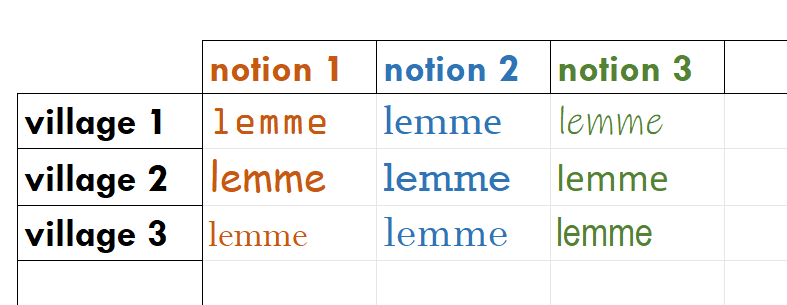
\includegraphics[width=0.6\textwidth]{dataframe}
\end{figure}

\subsection{Cartographie}

Nous avons donc des villages, des lemmes et des coordonnées de villages.
On trace ensuite des frontières avec les coordonnées des villages utilisant 
un même lemme pour une notion donnée et en fesant attention aux enclaves.

\begin{figure}[h]
\caption{Localisation des 6 lemmes de la notion "abeille"}
\centering
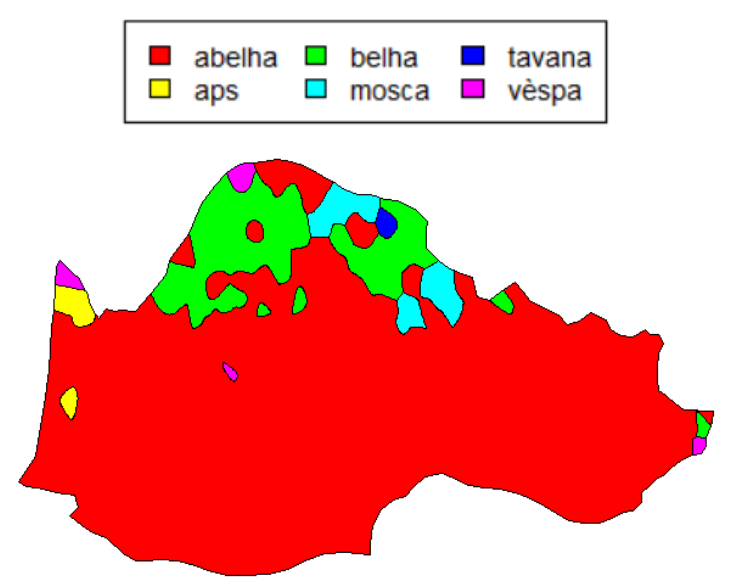
\includegraphics[width=0.6\textwidth]{notionAbeille}
\end{figure}


\subsection{Statistiques}
On connais donc pour chaque m2 de l'occitanie quel est la façon d'exprimer 
une notion. On souhaite maitenant mesurer mathématiquement la concordance avec 
des frontières géographiques. Cela nous permet de dire si tel ou tel frontière 
épousent les mêmes frontières. Pour ce faire il faut calculer la somme des aires 
qui intersectionne (en commun) de chaque lemme avec chaque section 
(exemple de section peut être le departement de l'aveyron).
Ce calcule retourne une matrice de contigence.
Tout nos calculs statistiques sont basées sur cette matrice.
Le calcul de Khi2, entropie, indice de localisation etc. sont des façon 
différentes de mesurer la dépendance et dispersion entre deux variables.

\begin{figure}[h]
\caption{Matrice de l’intersection des aires (km²) “Abeille” X régions dialectales}
\centering
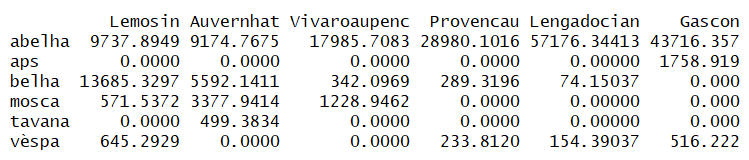
\includegraphics[width=0.6\textwidth]{matriceIntersection}
\end{figure}

\subsection{Dendrogramme}
Cette partie n'est pas terminé mais nous pouvons parler de son objectif.
On souhaite regrouper les lemmes qui sont le plus similaire, c'est à dire,
ceux ont une grande aire d'intersection dans les mêmes sections.
On pourrai donc passer de 20 lemmes par exemple à 6 lemmes, puis recontruire la 
carte avec que 6 couleurs. D'autre part, le clustering pourai theoriquement 
être utilisé pour recontruire des frontières géographiques en se basant 
uniquement sur les donnée geolinguistiques.

\begin{figure}[h]
\caption{Clustering des lemmes les plus similaires dans leurs dispersion géographique}
\centering
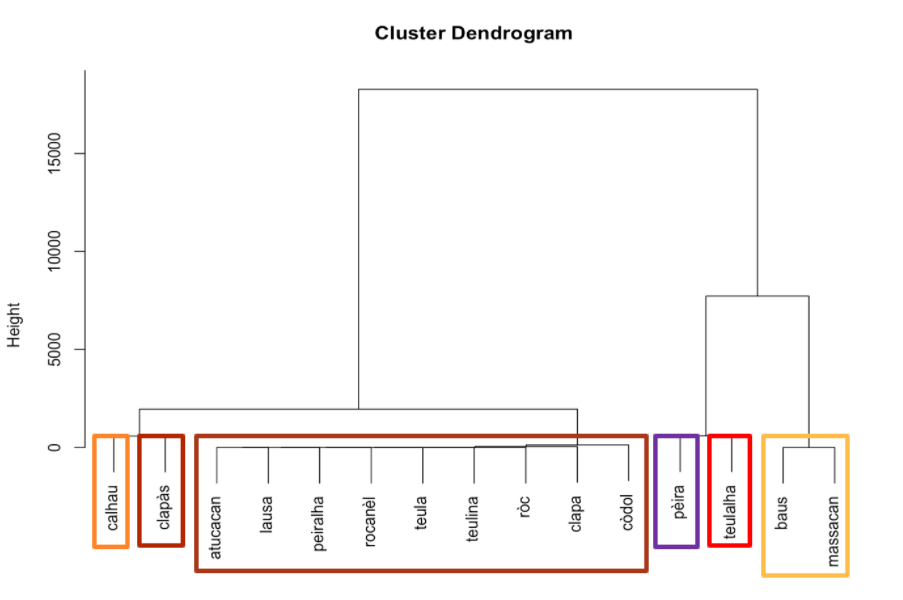
\includegraphics[width=0.6\textwidth]{dendrogramme}
\end{figure}


\section{Dévéloppement}

\subsection{Shiny}
Shiny permet de créer des dashboards en R. Il separe l'interface graphique et
le backend avec une partie ui et une partie server. 
Le deux parties sont connectés par des que vous avez a definir pour chaque 
element en entrée et ou sortie. L'idée générale et de contruire dans le UI 
la partie  saisie par le client.
Puis dans le serveur on fait appel aux fonction définie dans /R qui font les 
calculs et les graphiques etc.
Enfin l'UI définié la disposition des ces sorties sur la page.

\subsection{Golem}
golem est un package qui permet la création d'une application "Shiny" prête 
pour la production. golem, facilite le travail en équipe grâce a la séparation 
de l'application en modules, qui contiennent chaqu'un la partie UI et serveur. 
Ces modules peuvent être dévéloppés indépendament et intégrés rapidement.
Golem a plein de fonctionnalités tel que pour le deploiement qui facilite le 
travail du développeur. Et aussi pour gérér les dépendances en écrivant 
le NAMESPACE et DESCRIPTION.


\subsection{Dygraph}
dygraph est une bibliothèque de graphiques JavaScript. Nous l'utilisons pour un 
graphique de données temporelles interactif. Le jeux de données est à propos 
d'accidents de voiture en France. L'intégration avec l'application est s'est 
fait rapidement puisque nous lui avons attribué un module à part entière. 
Avec rétrospection, j'aurai plutôt préféré utilisé le package plotly car cela 
fait partie d'une famille d'outils d'analyse de données plus vaste que dygraph.
Nous avons perdu beaucoup de temp sur l'analyse de données des données accidents 
mais la grande mojorité n'a pas été inclu car il s'agissait d'analyse 
descriptives sans aucune composante intéractive et donc n'a pas d'intérêt pour 
une application shiny.

\begin{figure}[h]
\caption{Graphique de données chronologique et intéractif avec dygraph}
\centering
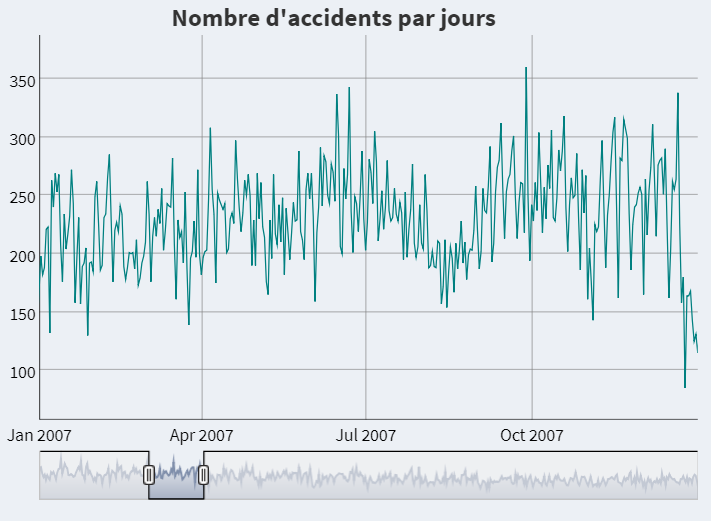
\includegraphics[width=0.6\textwidth]{dygraph}
\end{figure}
\newpage
\subsection{Git}
C'est le premier projet où j'utilise vraiment les fonctionnalités de 
gestionnaire de version et je suis agréablement impréssionné.


\subsection{Shinyapps io}
Le déploiment de l'application se fait facilement grâce a shinyapps.io et golem.  
shinyapps.io propose des services de déploiement d'application shiny en suivant 
un modèle freemium. Par conséquence leur service gratuit est bridé et peut 
créer des dysfonctionnements lorsque de la puissance de calcul est requis.


\subsection{Rcpp}
Nous obtenons en effet des problèmes d'optimisation quand l'application est 
déployé sur le service gratuit de shinyapps.io. Notament pour notre graphique 
interactif et lorsque on modifie le découpage géographie de la carte. Ces deux 
zones de dysfonctionnement sont notées par "1min de chargement" et provoquent 
une déconnexion du client. 

\begin{figure}[h]
\caption{Message d'erreure sur shinyapps.io lors du lancement d'un processus trop lourd}
\centering

\includegraphics[width=0.6\textwidth]{erreurServer}
\end{figure}

	L'optimisation de l'application est fortement 
conseillé si l'on passe en production car les temps de chargement sont parfois 
trop longs (même sur une machine puissante). Bien que le bridage soit 
partiellement responsable, il est possible de contourner ce problème par 
l'optimisation de l'application avec rcpp par exemple. Rcpp permet d'intégrer 
des fonctions écrites en C++ plûtot que R pour augmenter la vitesse du 
programme. Nous avons tenté d'utiliser Rcpp pour faire des calculs en relation 
avec 'collatz conjecture' qui dit que pour tout entier naturel supérieure à 1,
si on applique récusivement l'operation 3n+1 quand n est est impaire, et n/2 quand n est 
pair alors on fini toujours par tomber sur 1. Ça n'a jamais été démontré 
mathématiquement. Nous n'avons pas terminé cette partie mais nous aurions 
souhaité reproduire une visualisation comme celle ci dessous par exemple.

\begin{figure}[h]
\caption{Message d'erreure sur shinyapps.io lors du lancement d'un processus trop lourd}
\centering
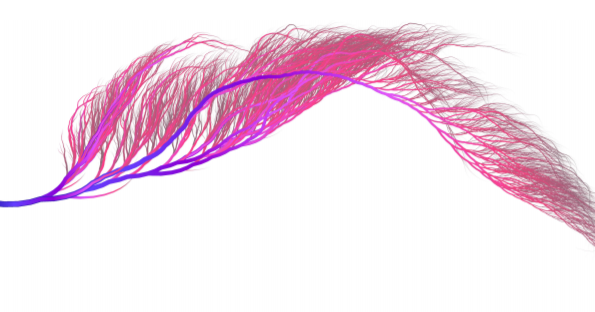
\includegraphics[width=0.6\textwidth]{collatz}
\end{figure}

\subsection{CSS}
dans inst->app->www->costum.css vous trouverez quelques styles pour la table 
statistque et du text. Grâce a golem, il n'y a pas de concurrence de 
balise html classe ou id.

\subsection{Roxygen2}
Pour la documentation des fonctions et de données de notre package nous 
utilisons roxygen2. De manière générale il suffit d'ajouter des commentaires 
avant votre fonction dans un format bien particulier mais facile a utiliser.
Dans ces commentaires, vous pouvez décrirer la fonction, ses paramètres et ses 
sorties etc. Une fois que vous avez fait le travail de correctement doccumenter 
votre package, roxygen2 s'occupe de créer le ficher de documentation r (.Rd).
C'est des fichier avec du latex.


\bibliographystyle{alpha}
\bibliography{bibs/sample}

\end{document}
